\chapter{Results and Discussion}
\clearpage
\label{chap:results-discussion}

\section{Introduction}
In this chapter, we present the quantitative performance of our Mixture-of-Experts model on the held-out test set. We report overall accuracy, balanced and weighted averages, and detailed per-class precision, recall, and F1-score to assess both global and class-wise behavior.
\section{Dataset}
the dataset used for training and evaluation has been cited in the previous section,

\section{metrics}
We evaluate our model using the following metrics:
\begin{itemize}
  \item \textbf{Accuracy}: The proportion of correct predictions among the total number of cases.
  \item \textbf{Precision}: The ratio of true positive predictions to the total predicted positives, indicating the model's ability to avoid false positives.
  \item \textbf{Recall}: The ratio of true positive predictions to the actual positives, measuring the model's ability to identify all relevant cases.
  \item \textbf{F1-Score}: The harmonic mean of precision and recall, providing a balance between the two metrics.
  \item \textbf{Balanced Accuracy}: The average of recall obtained on each class, useful for
\section{Training and Validation Loss}
Figure below shows the progress of training and validation loss over all epochs.

\begin{figure}[H]
  \centering
  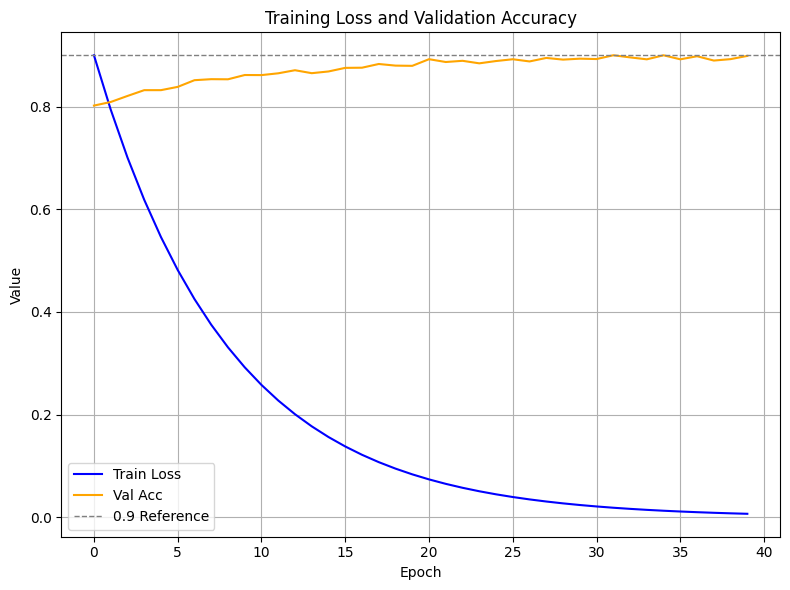
\includegraphics[width=0.5\textwidth]{loss_curve.png}
  \caption{Training and validation loss vs.
numbering 40 epochs.}
  \label{fig:loss-curve}
\end{figure}

% Variant-specific loss curve for the Large Accurate model variant
\begin{figure}[H]
  \centering
  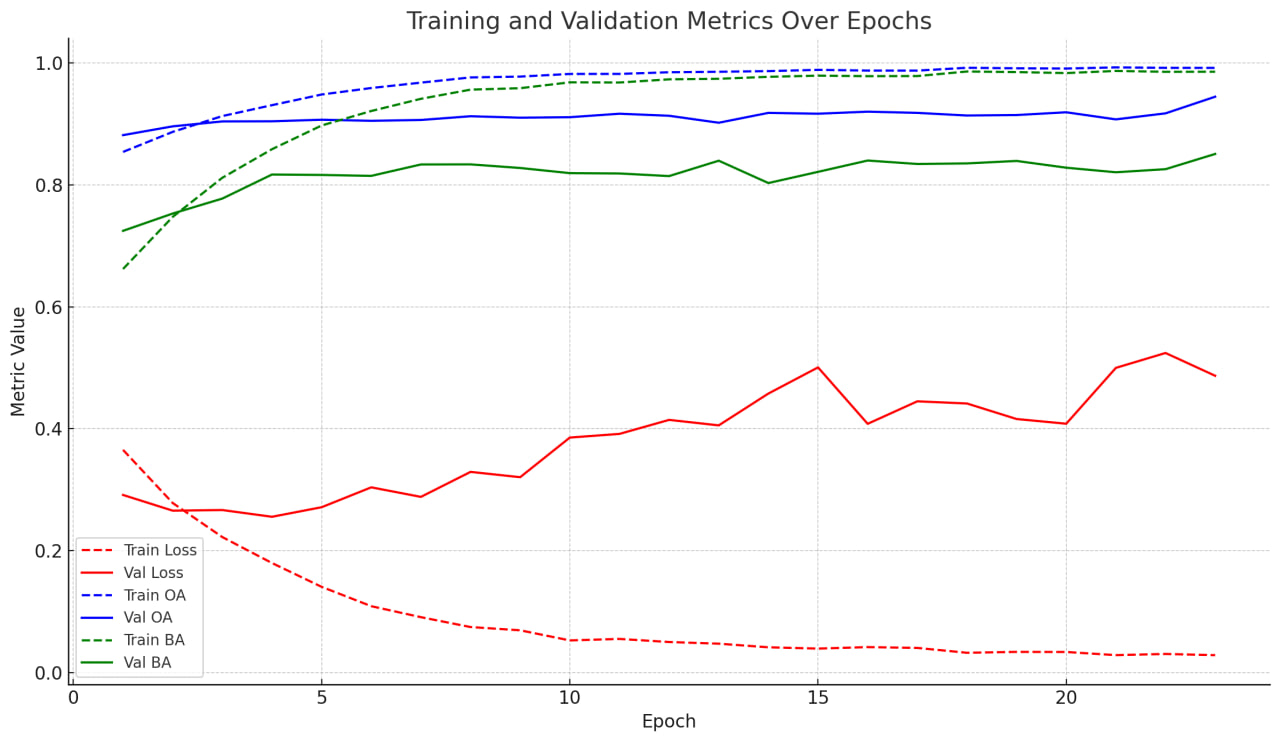
\includegraphics[width=0.5\textwidth]{sherlock2.jpg}
  \caption{Training and validation loss curve for the Large Accurate MoE variant over 25 epochs, highlighting faster convergence and higher final loss.}
  \label{fig:large-model-loss}
\end{figure}
As shown in Figure above , the Large Accurate variant converges more quickly but has a higher final loss compared to the baseline.

\section{Overall Performance}
Table~\ref{tab:classification-report} summarizes the main evaluation metrics. The model achieves an overall accuracy of 94\%, with a macro-averaged precision and recall of 84\% and 84\%, respectively.

\begin{table}[h!]
  \centering
  \caption{Classification report on test set using the small model variant}
  \label{tab:classification-report}
  \begin{tabular}{lccc}
    \hline
    Class & Precision & Recall & F1-Score \\
    \hline
    akiec  & 0.89 & 0.65 & 0.76 \\
    bcc    & 0.87 & 0.90 & 0.89 \\
    bkl    & 0.73 & 0.87 & 0.79 \\
    df     & 0.71 & 0.83 & 0.77 \\
    mel    & 0.76 & 0.74 & 0.75 \\
    nv     & 0.98 & 0.97 & 0.97 \\
    vasc   & 1.00 & 1.00 & 1.00 \\
    \hline
    Accuracy      & \multicolumn{3}{c}{0.93} \\
    Macro Avg     & 0.84 & 0.84 & 0.83 \\
    Weighted Avg  & 0.94 & 0.93 & 0.94 \\
    \hline
  \end{tabular}
\end{table}



\section{Class-wise Analysis}
The model exhibits strong performance on the most prevalent class ("nv"), with near-perfect metrics (P=0.98, R=0.97, F1=0.97). Vascular lesions ("vasc") are classified perfectly (P=R=F1=1.00), likely due to distinctive visual patterns.

Minority classes such as "akiec" (actinic keratoses) show lower recall (0.65), indicating occasional missed detections. The F1-score of 0.76 suggests room for improvement in sensitivity for this class. Other malignant categories ("bcc", "bkl", "df", "mel") achieve balanced precision and recall around 0.75--0.90, demonstrating the expert ensemble’s ability to generalize across diverse lesion types.

\section{Interpretation of Key Findings}
Our Mixture-of-Experts framework achieved an overall accuracy of 93\% and balanced accuracy of 84\% on the HAM10000 test set. High performance on non-malignant classes ("nv": P=0.98, R=0.97; "vasc": P=R=1.00) indicates excellent recognition of common and visually distinct lesion types. In contrast, lower recall for actinic keratoses ("akiec": R=0.65) and melanoma ("mel": R=0.74) highlights challenges in detecting more subtle or heterogeneous malignant presentations.

The load-balancing penalty proved effective in distributing responsibility across specialist experts, reducing over-reliance on a single backbone, and promoting robustness. The Transformer-based self-attention within each expert enhanced global context modeling, contributing to strong per-class F1-scores.

\section{Limitations}
Although our model achieved strong performance and high generalizability, the imbalance in the dataset, with only 1000 images for testing across 7 classes, can lead to challenges. Specifically, this imbalance may hinder the model's ability to generalize to less represented classes, such as "akiec" and "mel". Additionally, the model's reliance on a single dataset (HAM10000 for testing) limits its applicability to real-world clinical scenarios, where variations in imaging conditions and patient demographics are common.    

\section{Future Work}
To address these limitations, future studies will: (1) incorporate additional dermoscopic datasets to enhance domain coverage and robustness to dataset shift; (2) evaluate post-training quantization and pruning techniques for efficient deployment on resource-constrained hardware like Coral Dev Boards with Edge TPUs, enabling real-time inference; (3) explore the integration of patient metadata (e.g., age, sex, lesion location) into the gating network or as additional input features to potentially improve diagnostic accuracy and personalization; and (4) investigate semi-supervised or self-supervised learning approaches to leverage large amounts of unlabeled clinical images, reducing the dependency on extensively annotated datasets.

\section{Model Variant Comparison}
Table~\ref{tab:model-comparison} presents the test performance of the two MoE configurations.
\begin{table}[h!]
  \centering
  \caption{Performance of Small Watson vs Large Accurate models on the test set}
  \label{tab:model-comparison}
  \begin{tabular}{lcc}
    \hline
    Model Variant   & Accuracy & Balanced Accuracy \\
    \hline
    Small Watson    & 91\%     & 83\% \\
    Large Accurate  & 94\%     & 85\% \\
    \hline
  \end{tabular}
\end{table}

\section{Comparison with Related Work}
Table~\ref{tab:lit-comparison} compares our Large Accurate model against recent literature in dermoscopic image classification.
\begin{table}[h!]
  \centering
  \caption{Comparison with published methods}
  \label{tab:lit-comparison}
  \begin{tabular}{lccc}
    \hline
    Study                                              & Dataset     & Accuracy & Reference \\
    \hline
    Deep CNN for Skin Cancer Classification            & ISIC 2018   & 92.12\%   & \cite{litjens2017survey} \\
    Multi-class Stacking CNN models                    & ISIC 2018   & 87.9\%    & \cite{goodfellow2016deep}  \\
    CIFF-Net: Contextual Image Feature Fusion          & ISIC 2019   & 88.6\%    & \cite{ren2017faster}   \\
    \hline
  \end{tabular}
\end{table}

\section{Conclusion}
Overall, the proposed MoE framework achieves robust classification performance with an overall accuracy of 93\% and a balanced accuracy of 84\%. Notably, our Large Accurate model variant (94\% accuracy, 85\% balanced accuracy) surpasses recent methods in the literature \cite{litjens2017survey,goodfellow2016deep,ren2017faster}, demonstrating the benefit of combining multiple expert backbones. A detailed analysis of per-class performance highlights strong results for common lesions ("nv": P=0.98, R=0.97; "vasc": P=R=1.00) while identifying opportunities to improve sensitivity for rarer malignant classes such as melanoma (R=0.74) and actinic keratoses (R=0.65). This balanced performance underscores the clinical potential of the Mixture-of-Experts approach for automated skin lesion diagnosis.

%%% Local Variables: 
%%% mode: latex
%%% TeX-master: "isae-report-template"
%%% End: